%\section{intro}

The last type of PF particle candidates to be reconstructed are hadrons. Hadrons are composite particles made up of quarks and gluons are stopped by the HCAL. Some hadrons start showering in ECAL, however as seen in the previous chapter that ECAL is well calibrated for EM particles (electrons and photons), but not for hadrons.

a key feature of the hadronic showers is the fluctuation in showers generated by the same incident particle. these fluctuations from event to event could be in the fraction of energy lost as binding energy, particle type, particle multiplicity.

To accurately reconstruct hadron candidates, a correction for HCAL cluster energy needs to be applied after ECAL cluster calibration. This step is important for physics analysis since as mentioned before that pf candidates are used in reconstructing higher level physics objects.

This chapter similarly to the previous one introduced the ML method and datasets used in performing the PF HCAL cluster energy regression.  

\section{GNN} %source

GNN is a type of NN that is used to process data that can be represented as graphs. comparing to some kinds of NN, GNN can be applied on sparse data (thinly scattered like rechits). A graph consists of nodes which represent features of the objects, in our case will be represented by rechits and edges reflect the relationship between the rechit. information in GNN can be shared between neighbors. in our case seeing how rechits are connected, in clusters that represent one particle. (find related figure).

the vector feature of each node is transformed into messages (using dense layers) that will be sent to the neighbors (message passing) in this way each node will learn about its neighbors and itself. (add picture that shows massage passing) 



\section{datasets description}

The second part of the thesis focuses on the calibration charged hadrons pf clusters.
The data samples used for this calibration are single Pion gun.
They are centrally produced (reconstructed) MC samples, under 126X %CMSSW_12_6_4
, Run3 winter23, conditions. These samples are also available through DAS web page and they cover two ranges of E 2-200 GeV,200-500 GeV.  

Before using the data in training ML model, we need to prepare it according to the types of hadronic showers.
We have where H-hadrons are when the pion start showering in HCAL meaning the particles do not start a nuclear interaction in ECAL hadronic shower) and EH-hadrons are particles that start showering in ECAL. 


\section{PF cluster regression using DRN}

Hadronic showers in the CMS detector have both electromagnetic and hadronic components. These showers are not fully contained in the ECAL but extend to HCAL. The reconstructed energy of hadrons is the sum of all reconstructed hits (offline, PF reconstruct the RAW data) from the ECAL and HCAL. 

% DRN section. 

Cluster Energy is reconstructed using dynamic reduction network (DRN) (based on Graph neural network which mentioned in ML ch, %(Paper source , talk source)).
For a given bin of true energy we fit the distribution of total RAW energy with Gaussian then we obtain: mu (mean energy) and std deviation.

The DRN model maps input features onto a higher dimensional latent space and adds clustering and pooling steps to aggregate information. Where the input features this is energies (E) and (x,y,z) coordinates of individual cells (rechits - elected after dR matching) are provided to the model for training to the target. (E true/ E raw reconstructed energy using detector level calibration) and the output of the model is E pred (the energy reconstructed using DRN weights).

DRN architecture overview:  
step1: (Rechits) are the input for inputNet (FCNN - Fully Connected Network). 
step2: Graph Generation (KNN), EdgeConv, calculate edge weights, graph clustering (Graclus), graph pooling (add). 
Step3: Global pool (max).  
step4: output of outputNet is(E pred).

Other details related to the training, number of layers where input 3, aggregation 2, output 2, message passing 2. Other variable used in the training: batch size: 400, number of epochs trained 100, constant learning rate of 0.0001. The Loss functions used during training is defined as: (target - prediction)^2 / target

we checked different training target values: ratio, ratio flip, log (ratio flip), trueE.  
we can check the performance of the DRN training by plotting: loss vs epoch.

To test the DRN model results (applied on the testing data 20\% of the dataset) we calculate two quantities: first, average of calibrated E response = [ true energy (E true) - calibrated energy (E pre) ] / true energy in GeV for different true energy bins in specific eta range. The thinner the peak the better. 
Second, Energy resolution = std of (calibrated E response)/ true energy. These quantities are calculated for different regions (with different eta range): Barrel region. Endcap within the tracker region. Endcap outside the tracker region. (pt range from 1-300 GeV)  


\section{results}
we present the results of response and resolution (from DRN vs Chi2) in  both Barrel region and endcap region.

\subsection{EH Hadrons}
the presented results are for the training target ratioflip
\begin{figure}
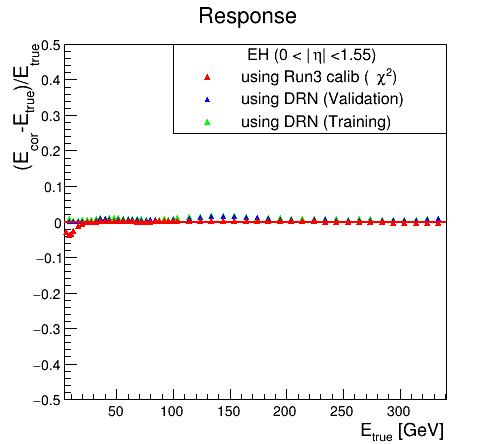
\includegraphics[width=0.495\textwidth]{./plots_pdf/HCAL_plots/Trained_target_ratioflip_0_500_10/pdf/EH_barrel/barrel_corrEtaBarrelEcalHcal.png}
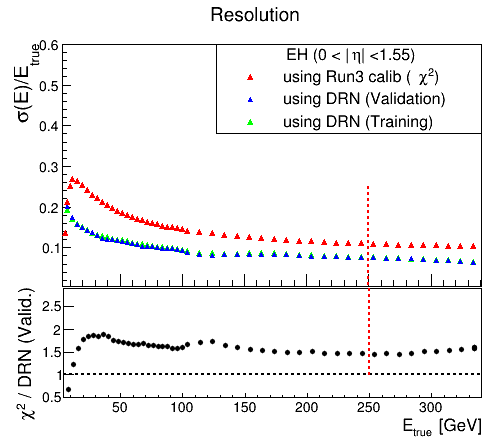
\includegraphics[width=0.495\textwidth]{./plots_pdf/HCAL_plots/Trained_target_ratioflip_0_500_10/pdf/EH_barrel/barrel_corrEtaBarrelEcalHcal_reso.png}
\caption{EH - barrel - target ratioflip}                                                                                                                                               
\end{figure}                                                                                                                                                                      

\begin{figure}                                                                                                                                                                   
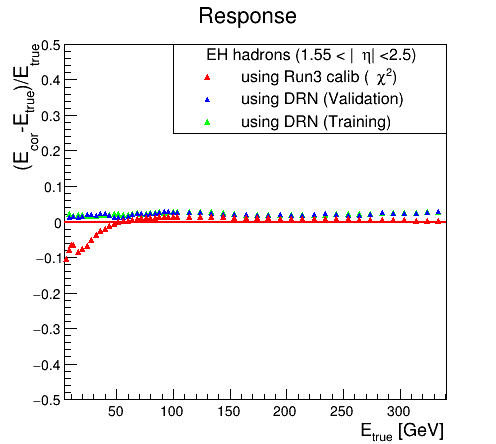
\includegraphics[width=0.495\textwidth]{./plots_pdf/HCAL_plots/Trained_target_ratioflip_0_500_10/pdf/EH_ec_in/EC_within_tracker_corrEtaEndcapEcalHcal.png}
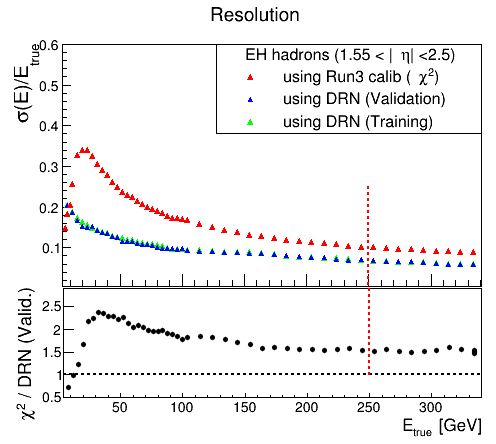
\includegraphics[width=0.495\textwidth]{./plots_pdf/HCAL_plots/Trained_target_ratioflip_0_500_10/pdf/EH_ec_in/EC_within_tracker_corrEtaEndcapEcalHcal_reso.png}
\caption{EH - endcap within tracker - target ratioflip}
\end{figure}


\begin{figure}
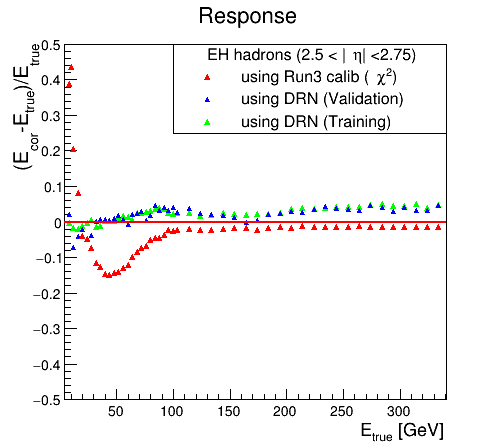
\includegraphics[width=0.495\textwidth]{./plots_pdf/HCAL_plots/Trained_target_ratioflip_0_500_10/pdf/EH_ec_out/EC_outside_tracker_corrEtaEndcapEcalHcal.png}
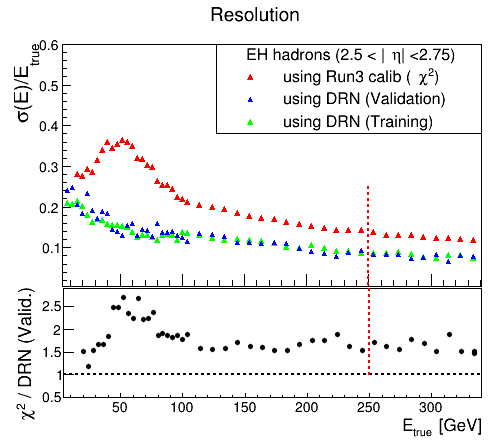
\includegraphics[width=0.495\textwidth]{./plots_pdf/HCAL_plots/Trained_target_ratioflip_0_500_10/pdf/EH_ec_out/EC_outside_tracker_corrEtaEndcapEcalHcal_reso.png}
\caption{EH - endcap outside the tracker - target ratioflip}
\end{figure}

\begin{figure}
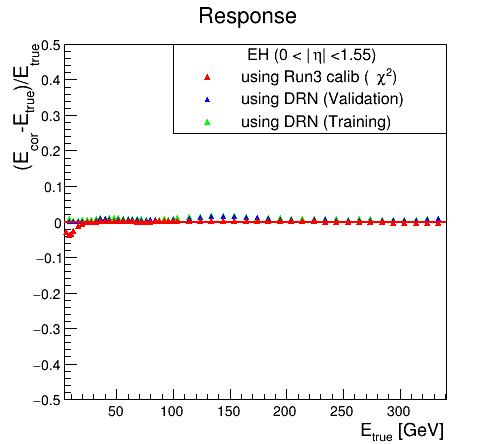
\includegraphics[width=0.495\textwidth]{./plots_pdf/HCAL_plots/Trained_target_ratioflip_0_500_10/pdf/EH_barrel/barrel_corrEtaBarrelEcalHcal.png}
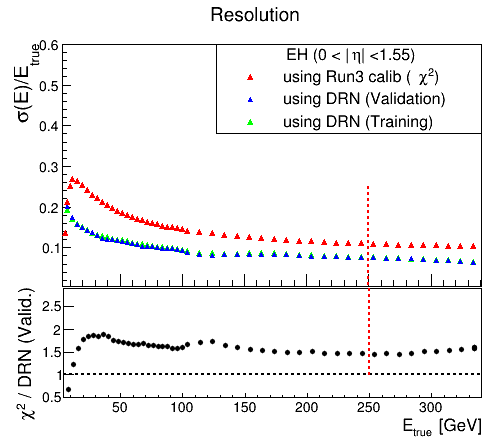
\includegraphics[width=0.495\textwidth]{./plots_pdf/HCAL_plots/Trained_target_ratioflip_0_500_10/pdf/EH_barrel/barrel_corrEtaBarrelEcalHcal_reso.png}
\caption{EH - barrel - target logratioflip}
\end{figure}

\begin{figure}
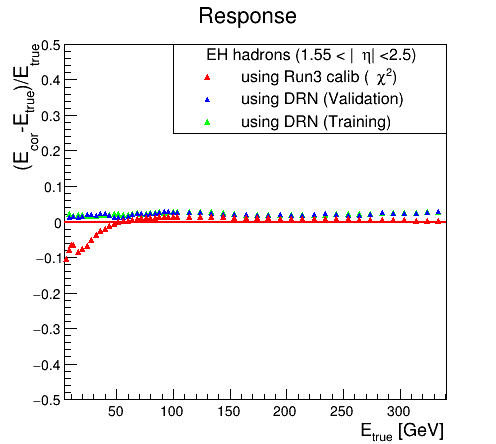
\includegraphics[width=0.495\textwidth]{./plots_pdf/HCAL_plots/Trained_target_ratioflip_0_500_10/pdf/EH_ec_in/EC_within_tracker_corrEtaEndcapEcalHcal.png}
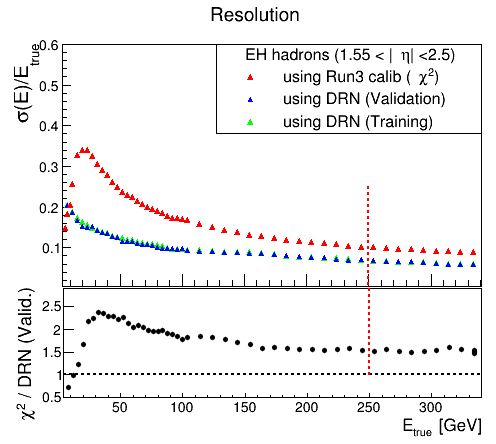
\includegraphics[width=0.495\textwidth]{./plots_pdf/HCAL_plots/Trained_target_ratioflip_0_500_10/pdf/EH_ec_in/EC_within_tracker_corrEtaEndcapEcalHcal_reso.png}
\caption{EH - endcap within tracker - target logratioflip}
\end{figure}


\begin{figure}
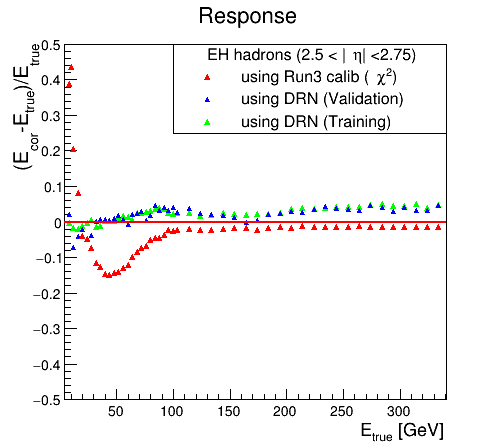
\includegraphics[width=0.495\textwidth]{./plots_pdf/HCAL_plots/Trained_target_ratioflip_0_500_10/pdf/EH_ec_out/EC_outside_tracker_corrEtaEndcapEcalHcal.png}
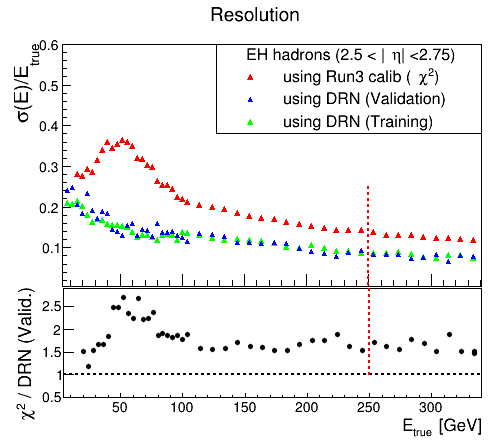
\includegraphics[width=0.495\textwidth]{./plots_pdf/HCAL_plots/Trained_target_ratioflip_0_500_10/pdf/EH_ec_out/EC_outside_tracker_corrEtaEndcapEcalHcal_reso.png}
\caption{EH - endcap outside the tracker - target logratioflip}
\end{figure}

\begin{figure}
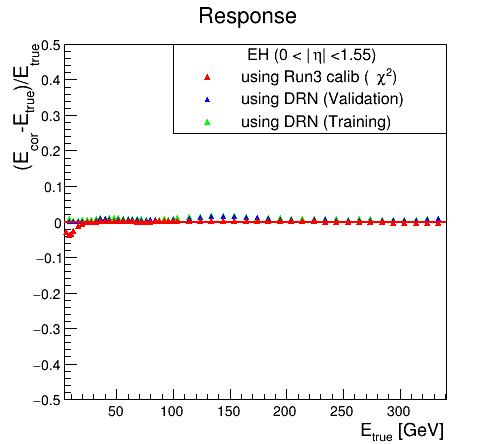
\includegraphics[width=0.495\textwidth]{./plots_pdf/HCAL_plots/Trained_target_ratioflip_0_500_10/pdf/EH_barrel/barrel_corrEtaBarrelEcalHcal.png}
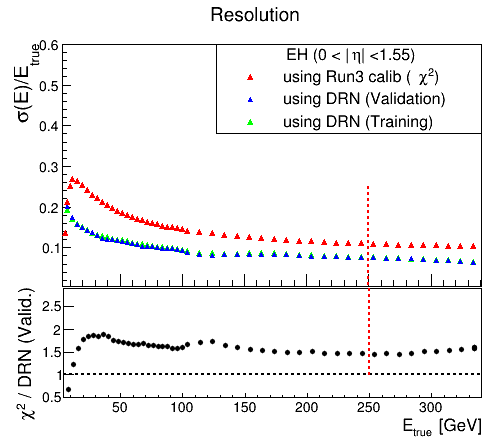
\includegraphics[width=0.495\textwidth]{./plots_pdf/HCAL_plots/Trained_target_ratioflip_0_500_10/pdf/EH_barrel/barrel_corrEtaBarrelEcalHcal_reso.png}
\caption{EH - barrel - target_ratio}                                                                                                                                               
\end{figure}                                                                                                                                                                      

\begin{figure}                                                                                                                                                                   
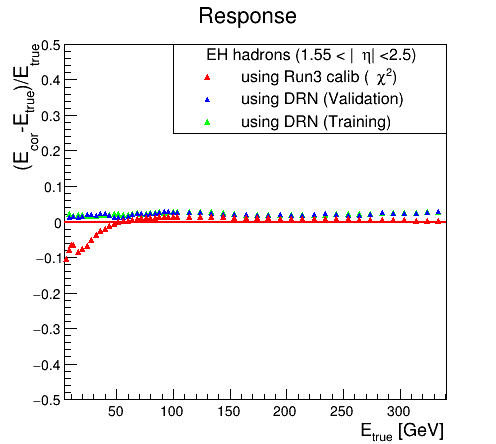
\includegraphics[width=0.495\textwidth]{./plots_pdf/HCAL_plots/Trained_target_ratioflip_0_500_10/pdf/EH_ec_in/EC_within_tracker_corrEtaEndcapEcalHcal.png}
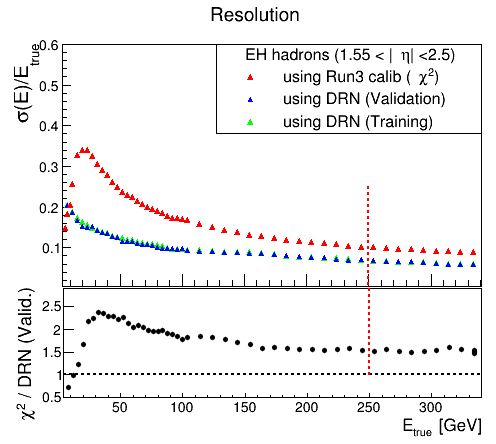
\includegraphics[width=0.495\textwidth]{./plots_pdf/HCAL_plots/Trained_target_ratioflip_0_500_10/pdf/EH_ec_in/EC_within_tracker_corrEtaEndcapEcalHcal_reso.png}
\caption{EH - endcap within tracker - target_ratio}
\end{figure}


\begin{figure}
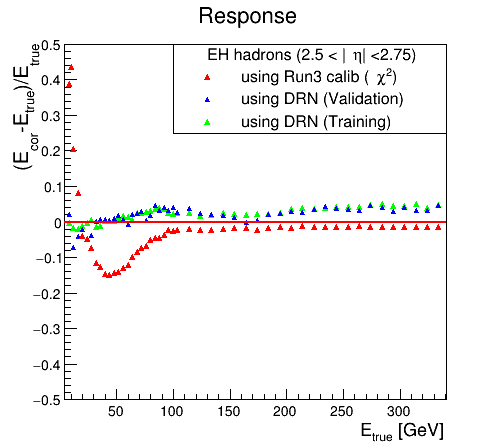
\includegraphics[width=0.495\textwidth]{./plots_pdf/HCAL_plots/Trained_target_ratioflip_0_500_10/pdf/EH_ec_out/EC_outside_tracker_corrEtaEndcapEcalHcal.png}
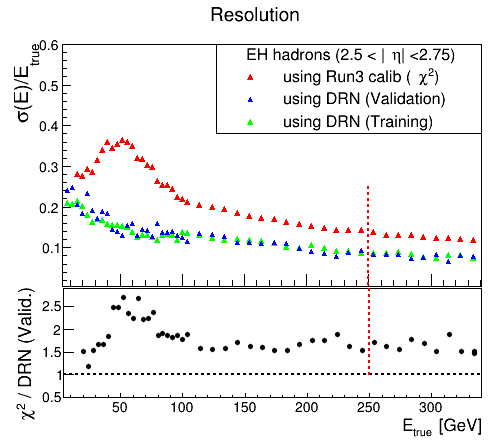
\includegraphics[width=0.495\textwidth]{./plots_pdf/HCAL_plots/Trained_target_ratioflip_0_500_10/pdf/EH_ec_out/EC_outside_tracker_corrEtaEndcapEcalHcal_reso.png}
\caption{EH - endcap outside the tracker - target_ratio}
\end{figure}

\begin{figure}
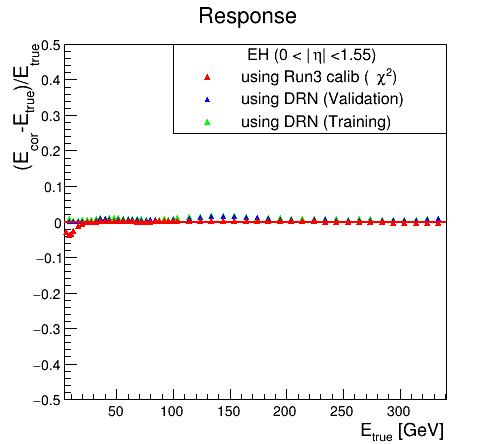
\includegraphics[width=0.495\textwidth]{./plots_pdf/HCAL_plots/Trained_target_ratioflip_0_500_10/pdf/EH_barrel/barrel_corrEtaBarrelEcalHcal.png}
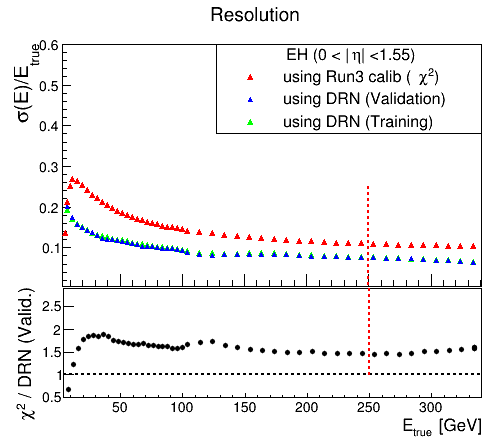
\includegraphics[width=0.495\textwidth]{./plots_pdf/HCAL_plots/Trained_target_ratioflip_0_500_10/pdf/EH_barrel/barrel_corrEtaBarrelEcalHcal_reso.png}
%\caption{EH - barrel - target trueE}
%\end{figure}

%\begin{figure}
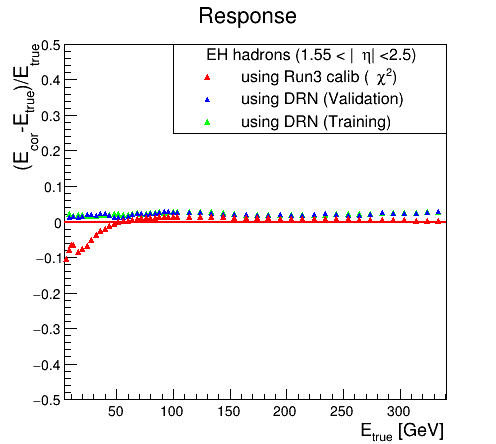
\includegraphics[width=0.495\textwidth]{./plots_pdf/HCAL_plots/Trained_target_ratioflip_0_500_10/pdf/EH_ec_in/EC_within_tracker_corrEtaEndcapEcalHcal.png}
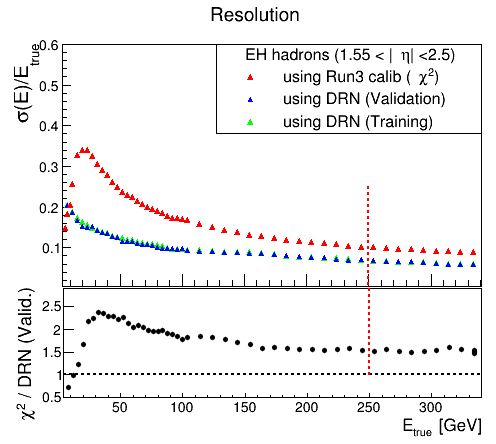
\includegraphics[width=0.495\textwidth]{./plots_pdf/HCAL_plots/Trained_target_ratioflip_0_500_10/pdf/EH_ec_in/EC_within_tracker_corrEtaEndcapEcalHcal_reso.png}
%\caption{EH - endcap within tracker - target trueE}
%\end{figure}


%\begin{figure}
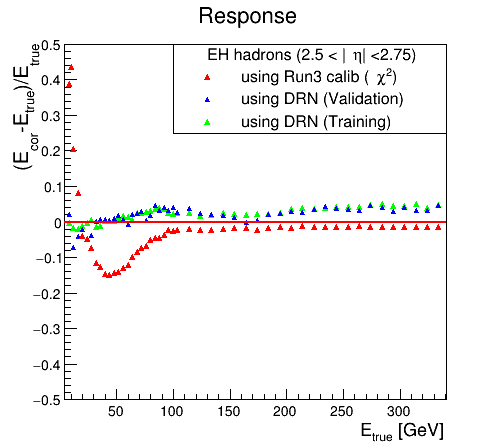
\includegraphics[width=0.495\textwidth]{./plots_pdf/HCAL_plots/Trained_target_ratioflip_0_500_10/pdf/EH_ec_out/EC_outside_tracker_corrEtaEndcapEcalHcal.png}
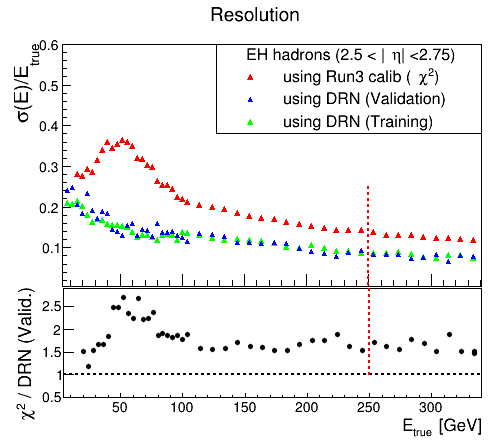
\includegraphics[width=0.495\textwidth]{./plots_pdf/HCAL_plots/Trained_target_ratioflip_0_500_10/pdf/EH_ec_out/EC_outside_tracker_corrEtaEndcapEcalHcal_reso.png}
\caption{EH - (top) barrel, (middle) endcap within tracker, (bottom) endcap outside the tracker - target trueE}
\label{fig:EH_trueE}
\end{figure}


\subsection{H hadrons}
\begin{figure}
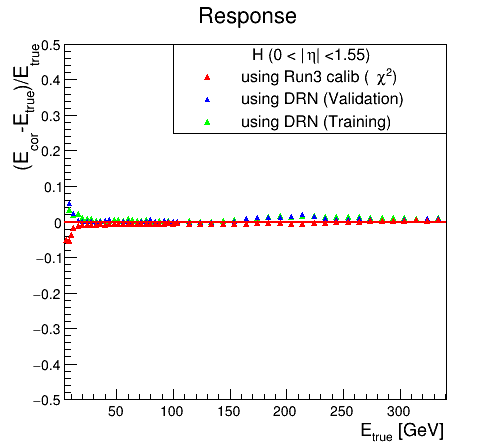
\includegraphics[width=0.495\textwidth]{./plots_pdf/HCAL_plots/Trained_target_ratioflip_0_500_10/pdf/H_barrel/barrel_corrEtaBarrelHcal.png}
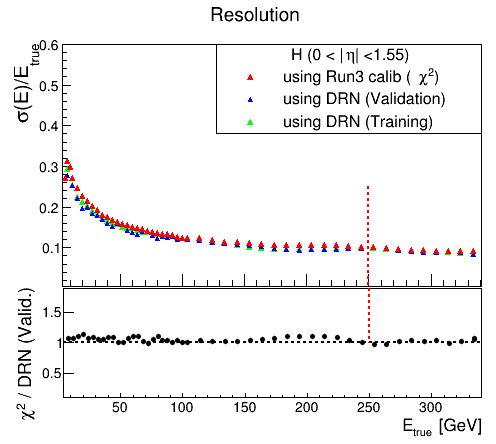
\includegraphics[width=0.495\textwidth]{./plots_pdf/HCAL_plots/Trained_target_ratioflip_0_500_10/pdf/H_barrel/barrel_corrEtaBarrelHcal_reso.png}

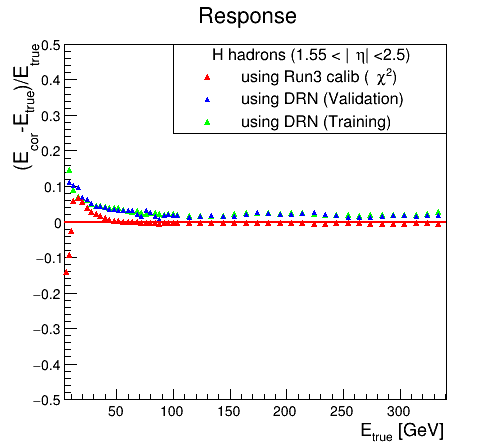
\includegraphics[width=0.495\textwidth]{./plots_pdf/HCAL_plots/Trained_target_ratioflip_0_500_10/pdf/H_ec_in/EC_within_tracker_corrEtaEndcapHcal.png}
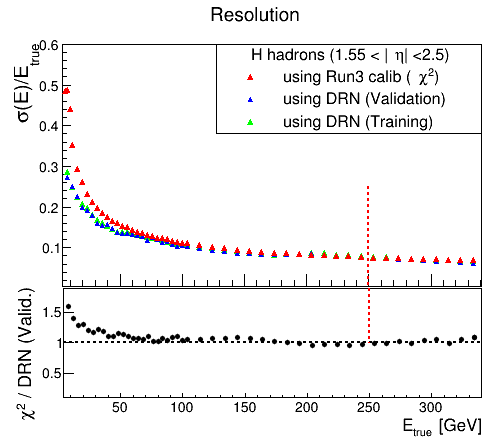
\includegraphics[width=0.495\textwidth]{./plots_pdf/HCAL_plots/Trained_target_ratioflip_0_500_10/pdf/H_ec_in/EC_within_tracker_corrEtaEndcapHcal_reso.png}

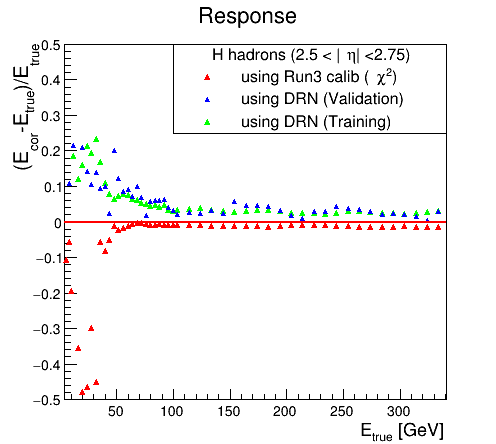
\includegraphics[width=0.495\textwidth]{./plots_pdf/HCAL_plots/Trained_target_ratioflip_0_500_10/pdf/H_ec_out/EC_outside_tracker_corrEtaEndcapHcal.png}
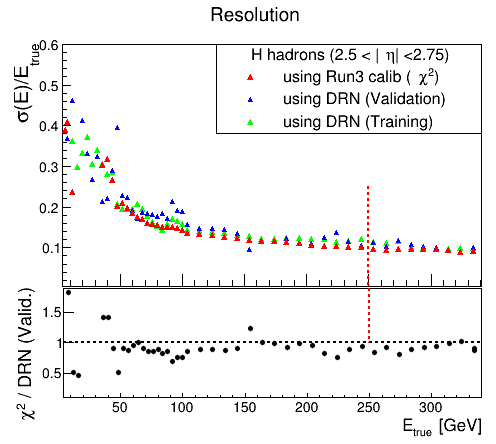
\includegraphics[width=0.495\textwidth]{./plots_pdf/HCAL_plots/Trained_target_ratioflip_0_500_10/pdf/H_ec_out/EC_outside_tracker_corrEtaEndcapHcal_reso.png}

\caption[Energy response (resolution) of the PF H-hadron cluster training traget ratioflip]{H - (top) barrel , (middle) endcap within tracker, (bottom) endcap outside the tracker - target ratioflip}
\label{fig:H_ratioflip}
\end{figure}

\begin{figure}
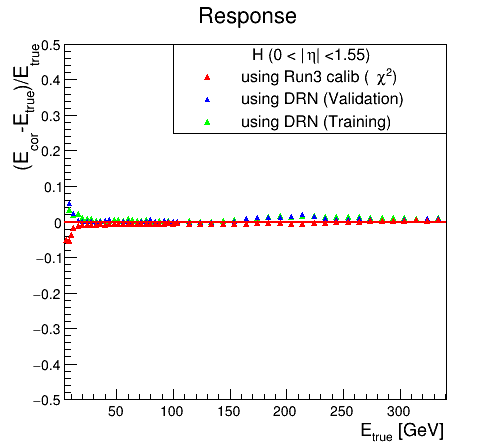
\includegraphics[width=0.495\textwidth]{./plots_pdf/HCAL_plots/Trained_target_ratioflip_0_500_10/pdf/H_barrel/barrel_corrEtaBarrelHcal.png}
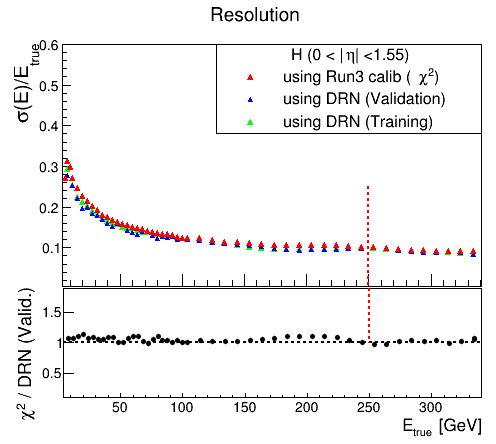
\includegraphics[width=0.495\textwidth]{./plots_pdf/HCAL_plots/Trained_target_ratioflip_0_500_10/pdf/H_barrel/barrel_corrEtaBarrelHcal_reso.png}
\caption{H - barrel - target_logratioflip}                                                                                                                                               
\end{figure}


\begin{figure}                                                                                                                                                               
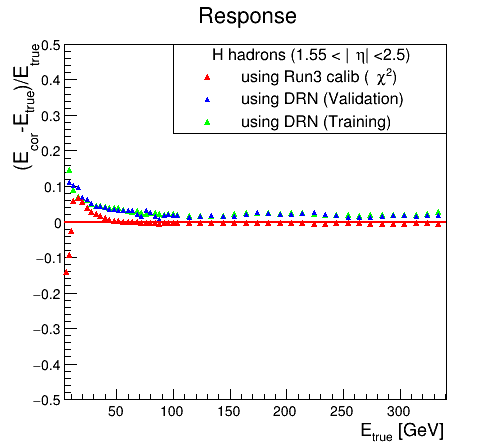
\includegraphics[width=0.495\textwidth]{./plots_pdf/HCAL_plots/Trained_target_ratioflip_0_500_10/pdf/H_ec_in/EC_within_tracker_corrEtaEndcapHcal.png}
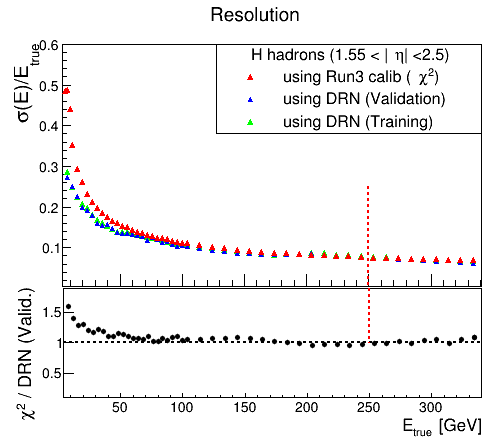
\includegraphics[width=0.495\textwidth]{./plots_pdf/HCAL_plots/Trained_target_ratioflip_0_500_10/pdf/H_ec_in/EC_within_tracker_corrEtaEndcapHcal_reso.png}
\caption{H - endcap within tracker - target_logratioflip}
\end{figure}


\begin{figure}
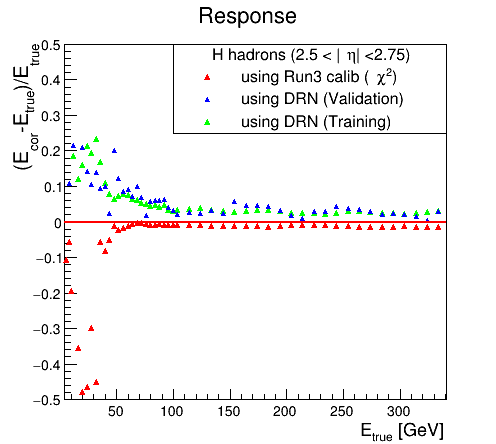
\includegraphics[width=0.495\textwidth]{./plots_pdf/HCAL_plots/Trained_target_ratioflip_0_500_10/pdf/H_ec_out/EC_outside_tracker_corrEtaEndcapHcal.png}
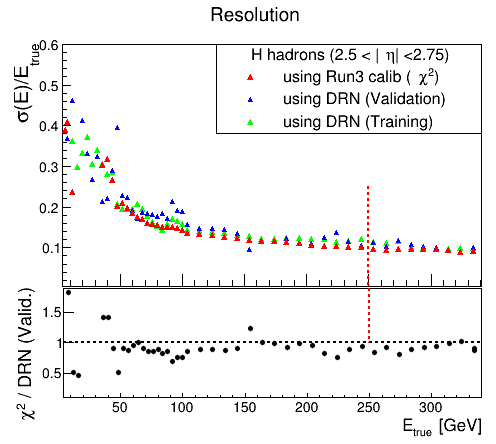
\includegraphics[width=0.495\textwidth]{./plots_pdf/HCAL_plots/Trained_target_ratioflip_0_500_10/pdf/H_ec_out/EC_outside_tracker_corrEtaEndcapHcal_reso.png}
\caption{H - endcap outside the tracker - target_logratioflip}
\end{figure}

\begin{figure}
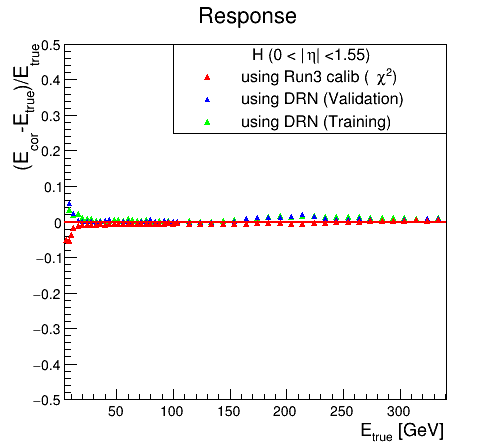
\includegraphics[width=0.495\textwidth]{./plots_pdf/HCAL_plots/Trained_target_ratioflip_0_500_10/pdf/H_barrel/barrel_corrEtaBarrelHcal.png}
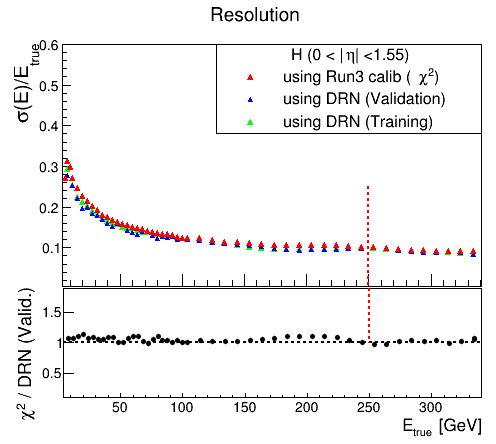
\includegraphics[width=0.495\textwidth]{./plots_pdf/HCAL_plots/Trained_target_ratioflip_0_500_10/pdf/H_barrel/barrel_corrEtaBarrelHcal_reso.png}
%\caption{H - barrel - target ratio}
%\end{figure}


%\begin{figure}
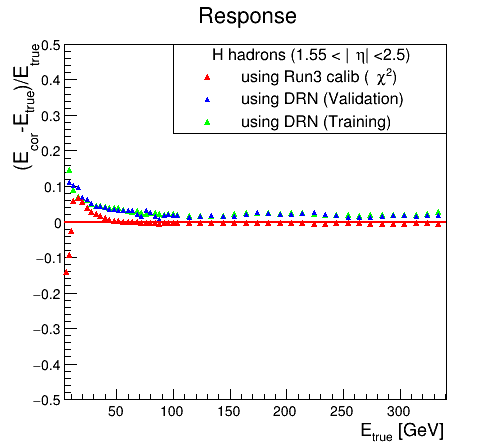
\includegraphics[width=0.495\textwidth]{./plots_pdf/HCAL_plots/Trained_target_ratioflip_0_500_10/pdf/H_ec_in/EC_within_tracker_corrEtaEndcapHcal.png}
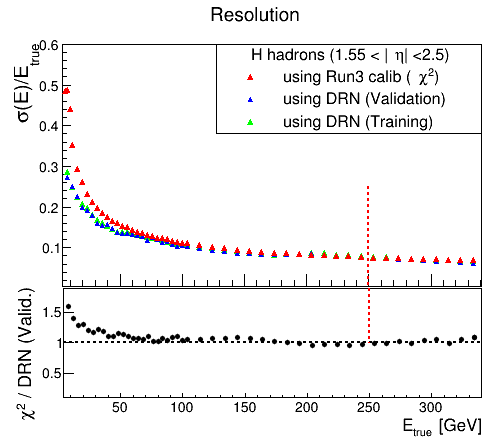
\includegraphics[width=0.495\textwidth]{./plots_pdf/HCAL_plots/Trained_target_ratioflip_0_500_10/pdf/H_ec_in/EC_within_tracker_corrEtaEndcapHcal_reso.png}
%\caption{H - endcap within tracker - target ratio}
%\end{figure}


%\begin{figure}
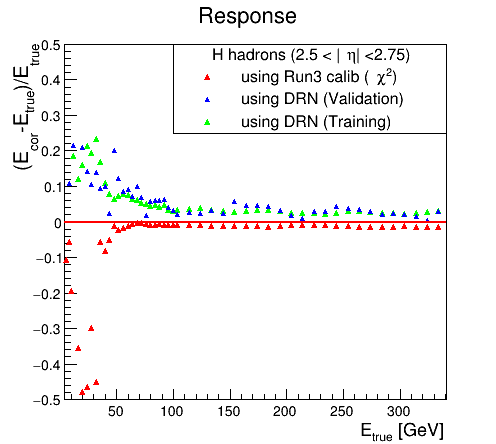
\includegraphics[width=0.495\textwidth]{./plots_pdf/HCAL_plots/Trained_target_ratioflip_0_500_10/pdf/H_ec_out/EC_outside_tracker_corrEtaEndcapHcal.png}
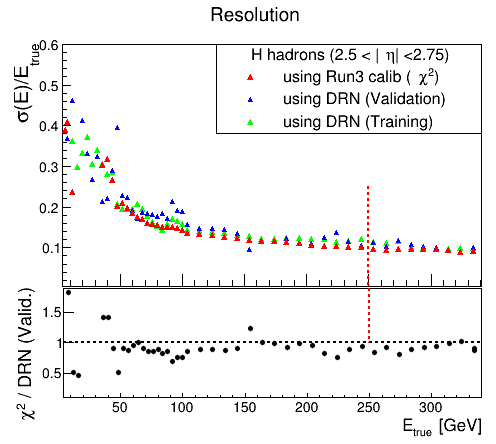
\includegraphics[width=0.495\textwidth]{./plots_pdf/HCAL_plots/Trained_target_ratioflip_0_500_10/pdf/H_ec_out/EC_outside_tracker_corrEtaEndcapHcal_reso.png}
\caption{H - (top) barrel, (middle) endcap within tracker, (bottom) endcap outside the tracker - target ratio}
\end{figure}

\begin{figure}
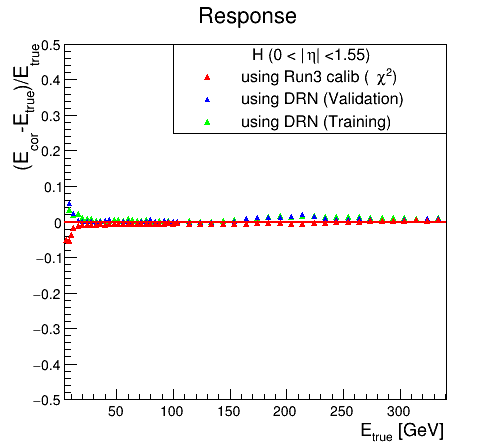
\includegraphics[width=0.495\textwidth]{./plots_pdf/HCAL_plots/Trained_target_ratioflip_0_500_10/pdf/H_barrel/barrel_corrEtaBarrelHcal.png}
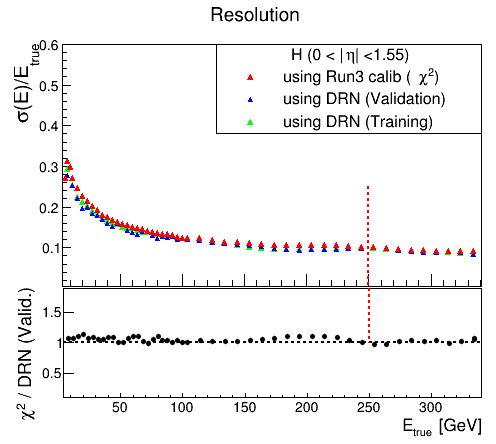
\includegraphics[width=0.495\textwidth]{./plots_pdf/HCAL_plots/Trained_target_ratioflip_0_500_10/pdf/H_barrel/barrel_corrEtaBarrelHcal_reso.png}
\caption{H - barrel - target_trueE}                                                                                                                                               
\end{figure}


\begin{figure}                                                                                                                                                               
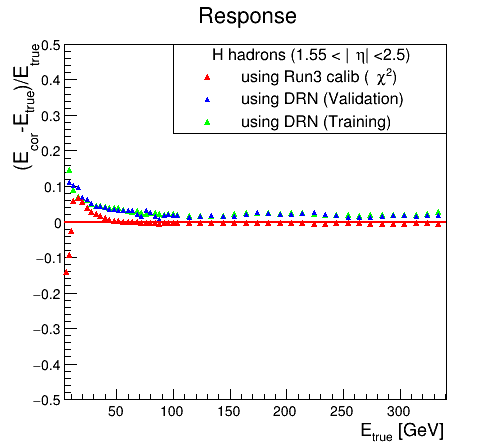
\includegraphics[width=0.495\textwidth]{./plots_pdf/HCAL_plots/Trained_target_ratioflip_0_500_10/pdf/H_ec_in/EC_within_tracker_corrEtaEndcapHcal.png}
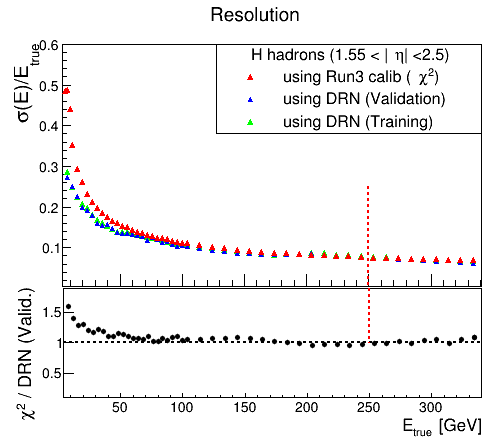
\includegraphics[width=0.495\textwidth]{./plots_pdf/HCAL_plots/Trained_target_ratioflip_0_500_10/pdf/H_ec_in/EC_within_tracker_corrEtaEndcapHcal_reso.png}
\caption{H - endcap within tracker - target_trueE}
\end{figure}


\begin{figure}
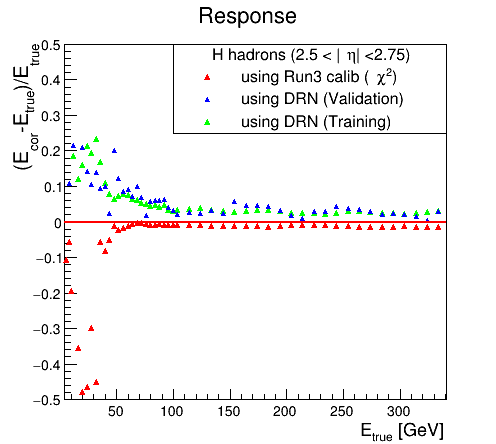
\includegraphics[width=0.495\textwidth]{./plots_pdf/HCAL_plots/Trained_target_ratioflip_0_500_10/pdf/H_ec_out/EC_outside_tracker_corrEtaEndcapHcal.png}
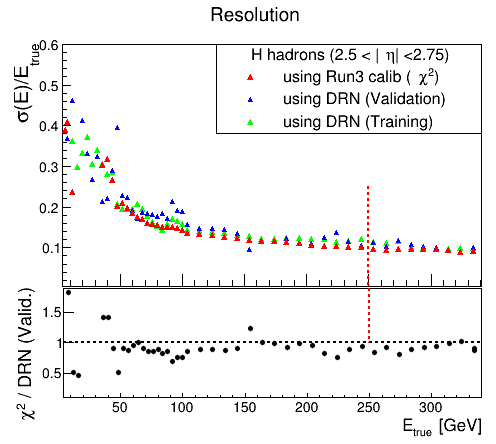
\includegraphics[width=0.495\textwidth]{./plots_pdf/HCAL_plots/Trained_target_ratioflip_0_500_10/pdf/H_ec_out/EC_outside_tracker_corrEtaEndcapHcal_reso.png}
\caption{H - endcap outside the tracker - target_trueE}
\end{figure}

